The aim of this project is to analyze a dataset collected from NBA Rookies' games \cite{NBARS:2016}. This set contains 1340 samples, each one described by the 21 features listed below: 
\begin{itemize}
	\item Name of the player (Name): string;
	\item Number of games played (GP): discrete positive variable;
	\item Minutes played per game (MIN): continuous positive variable;
	\item Points scored per game (PTS): continuous positive variable;
	\item Field goals made per game (FGM): continuous positive variable;
	\item Field goals attempts per game (FGA): continuous positive  variable;
	\item Field goals percent per game (FG\%): continuous positive variable;
	\item 3 point shots made per game (3P MADE): continuous positive variable;
	\item 3 points shots attempts per game (3PA): continuous positive variable;
	\item 3 point shots percent per game (3P\%): continuous positive variable;
	\item Free throws made per game (FTM): continuous positive variable;
	\item Free throws attempts per game (FTA): continuous positive variable;
	\item Free throws percent per game (FT\%): continuous positive variable;
	\item Number of offensive rebounds per game (OREB): continuous positive variable;
	\item Number of defensive rebounds per game (DREB): continuous positive variable;
	\item Number of rebounds per game (REB): continuous positive variable;
	\item Number of assists per game (AST): continuous positive variable;
	\item Number of steals per game (STL): continuous positive variable;
	\item Number of blocks per game (BLK): continuous positive variable;
	\item Number of turnovers per game (TOV): continuous positive variable;
	\item Output variable (TARGET\_5Yrs): binary variable (1 if career duration is greater than or equal to 5 years, 0 otherwise).\\
\end{itemize} 

The histograms of the 19 useful regressors are shown in \Fig~\ref{fig:Histograms}.
\begin{figure}[H]
	\centering
	\begin{subfigure}{.3\textwidth}
		\centering
		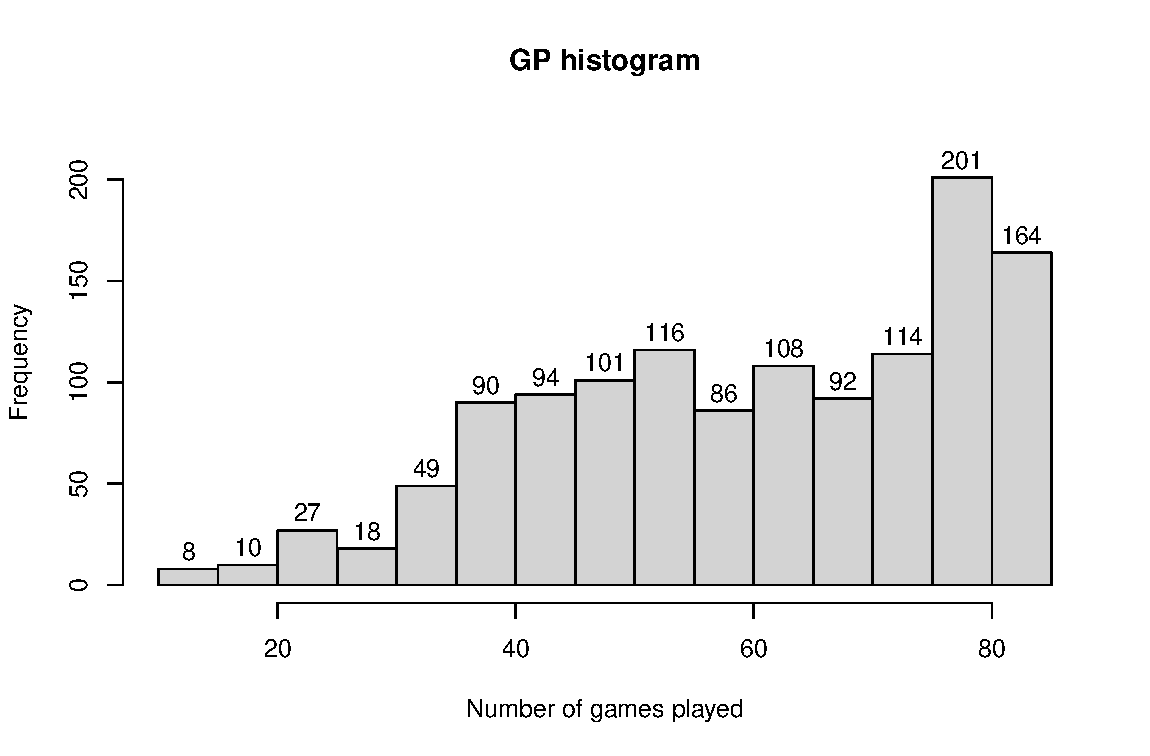
\includegraphics[width=0.5\linewidth]{ImageFiles/Histograms/histogram_gp.pdf}
		\caption{}
		\label{fig:HistGP}
	\end{subfigure}%
	\begin{subfigure}{.3\textwidth}
		\centering
		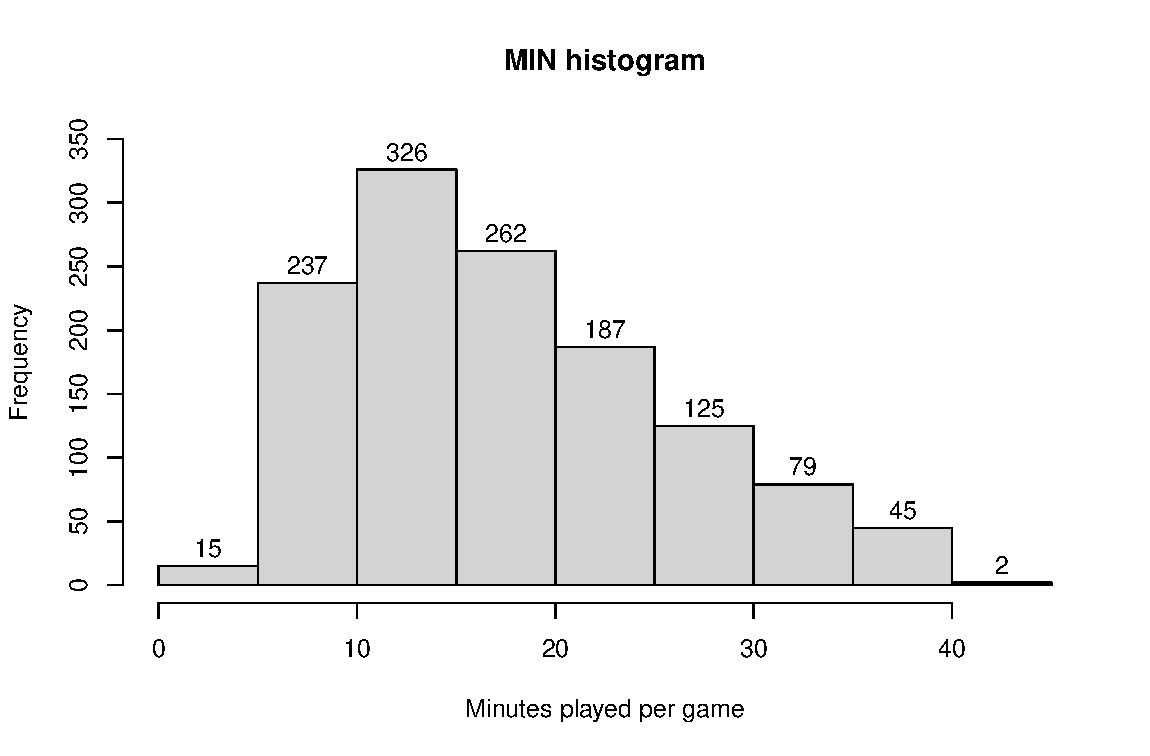
\includegraphics[width=0.5\linewidth]{ImageFiles/Histograms/histogram_min.pdf}
		\caption{}
		\label{fig:HistMIN}
	\end{subfigure}%
	\begin{subfigure}{.3\textwidth}
		\centering
		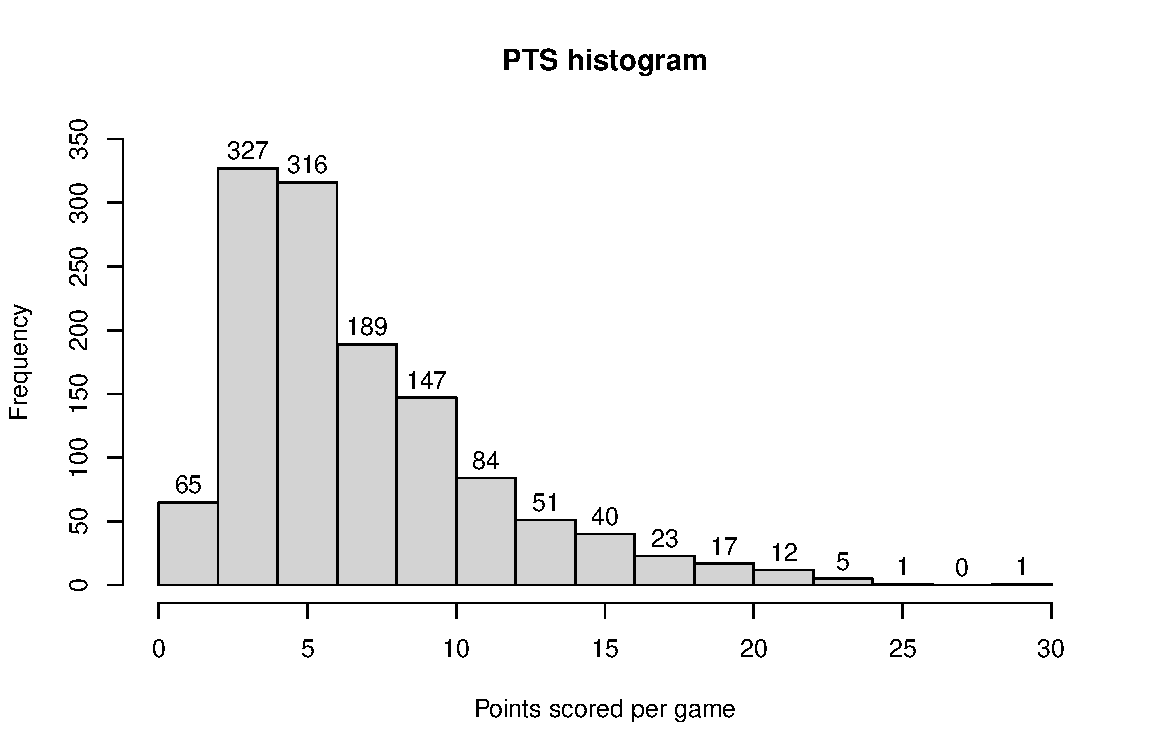
\includegraphics[width=0.5\linewidth]{ImageFiles/Histograms/histogram_pts.pdf}
		\caption{}
		\label{fig:HistPTS}
	\end{subfigure}
	\begin{subfigure}{.3\textwidth}
		\centering
		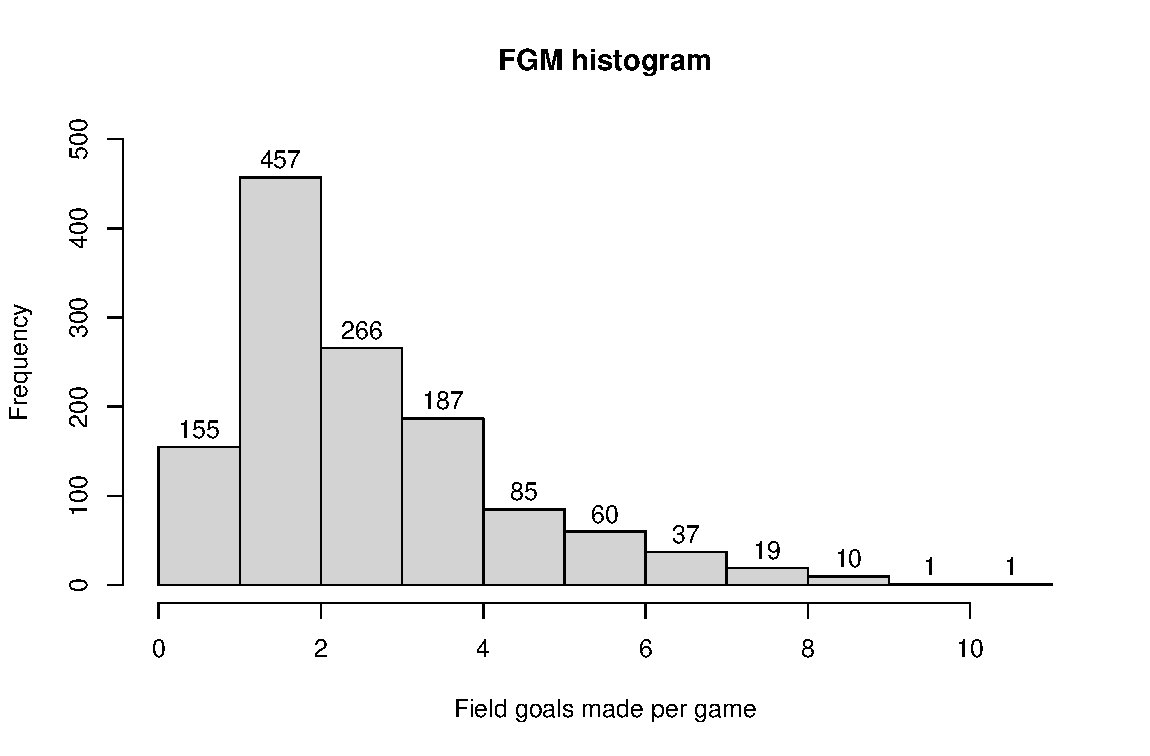
\includegraphics[width=0.5\linewidth]{ImageFiles/Histograms/histogram_fgm.pdf}
		\caption{}
		\label{fig:HistFGM}
	\end{subfigure}%
	\begin{subfigure}{.3\textwidth}
		\centering
		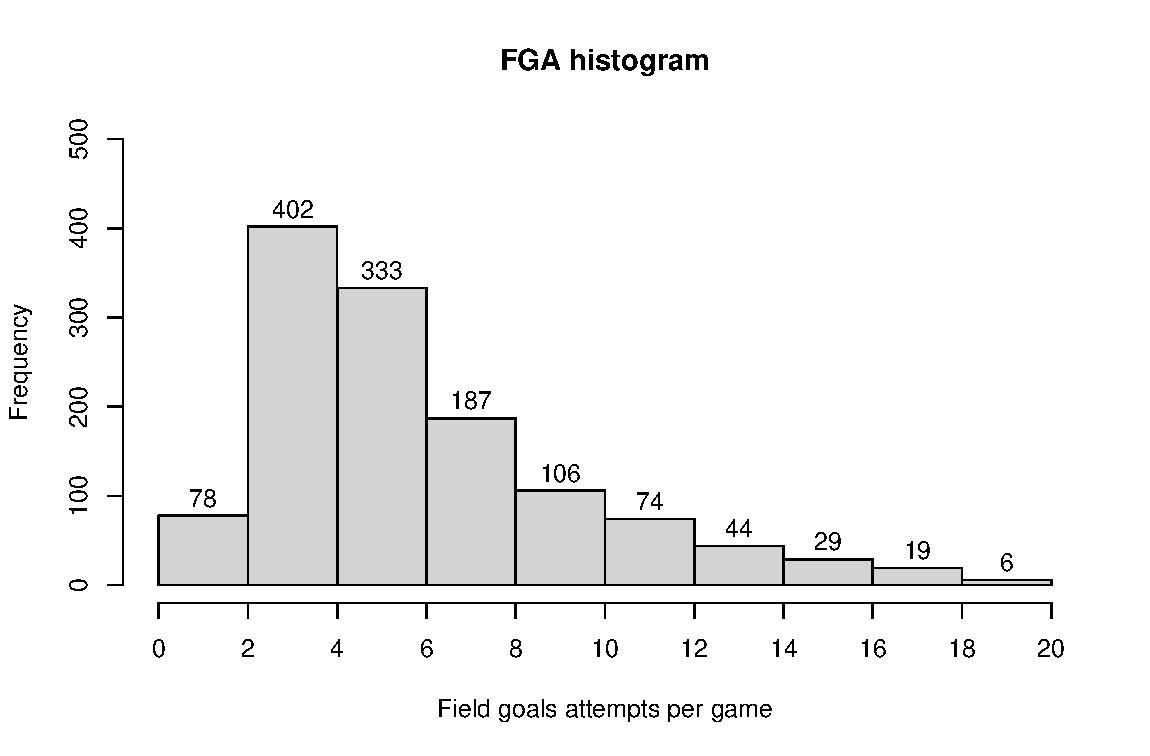
\includegraphics[width=0.5\linewidth]{ImageFiles/Histograms/histogram_fga.pdf}
		\caption{}
		\label{fig:HistFGA}
	\end{subfigure}%
	\begin{subfigure}{.3\textwidth}
		\centering
		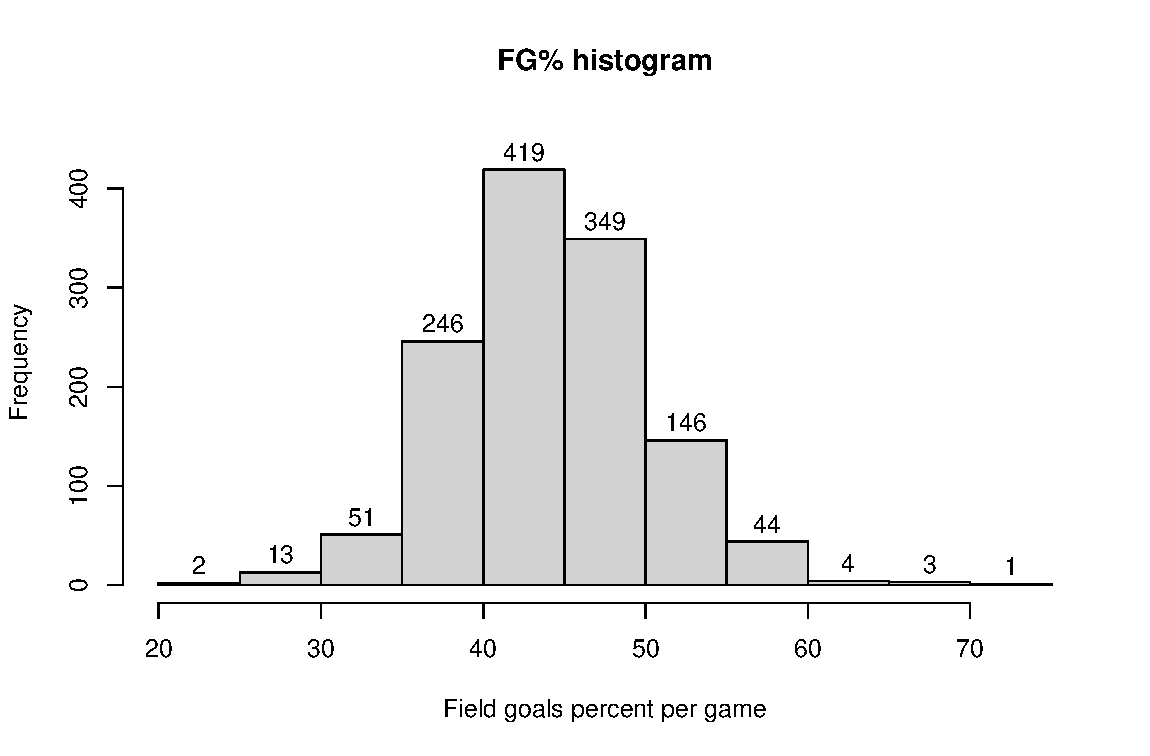
\includegraphics[width=0.5\linewidth]{ImageFiles/Histograms/histogram_fg.pdf}
		\caption{}
		\label{fig:HistFG}
	\end{subfigure}
	\begin{subfigure}{.3\textwidth}
		\centering
		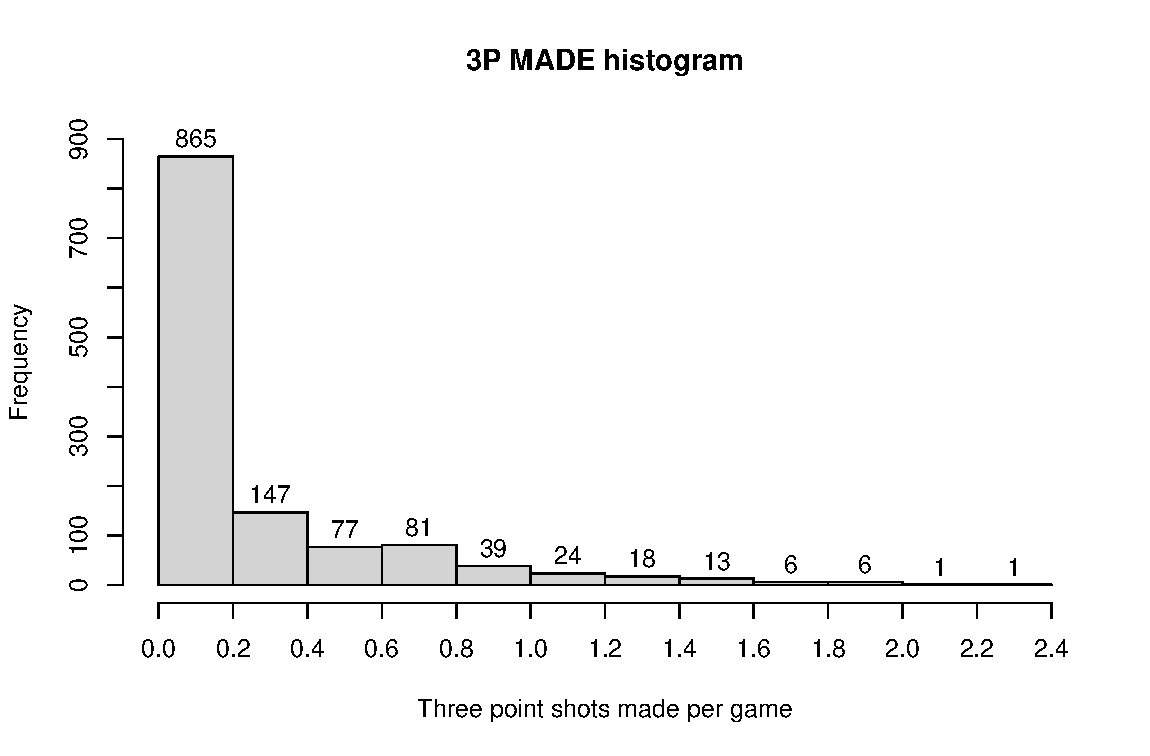
\includegraphics[width=0.5\linewidth]{ImageFiles/Histograms/histogram_x3pmade.pdf}
		\caption{}
		\label{fig:HistX3PMADE}
	\end{subfigure}%
	\begin{subfigure}{.3\textwidth}
		\centering
		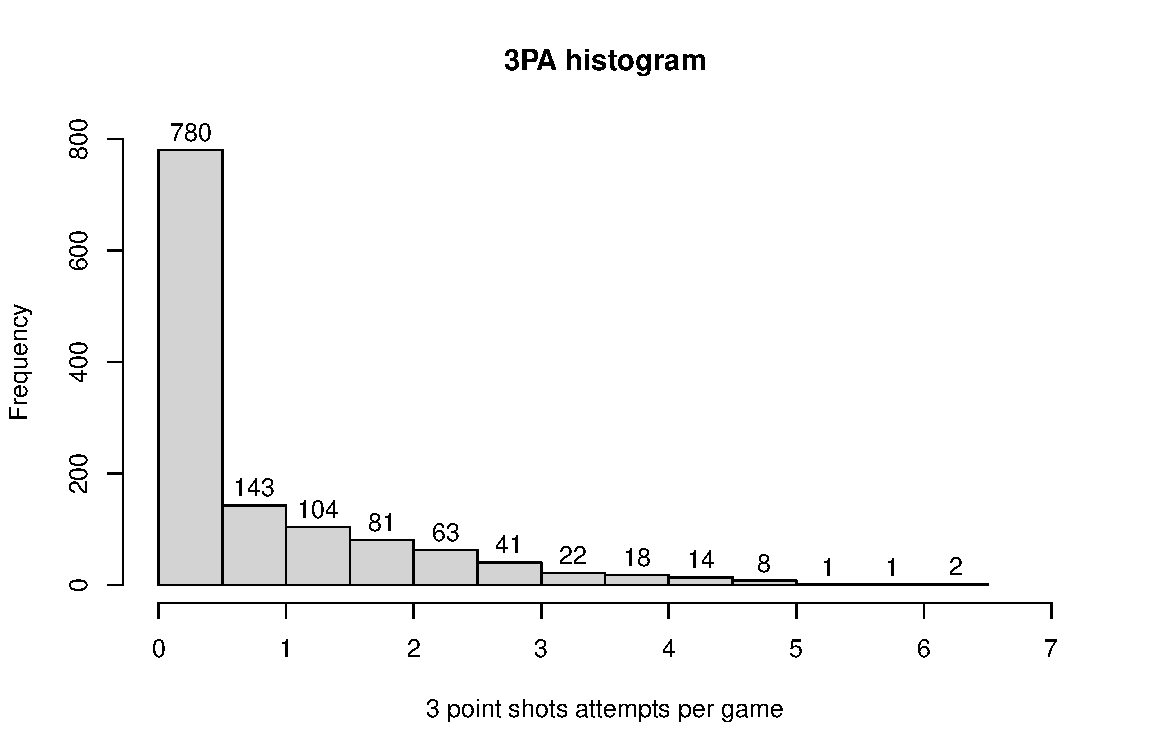
\includegraphics[width=0.5\linewidth]{ImageFiles/Histograms/histogram_x3pa.pdf}
		\caption{}
		\label{fig:HistX3PA}
	\end{subfigure}%
	\begin{subfigure}{.3\textwidth}
		\centering
		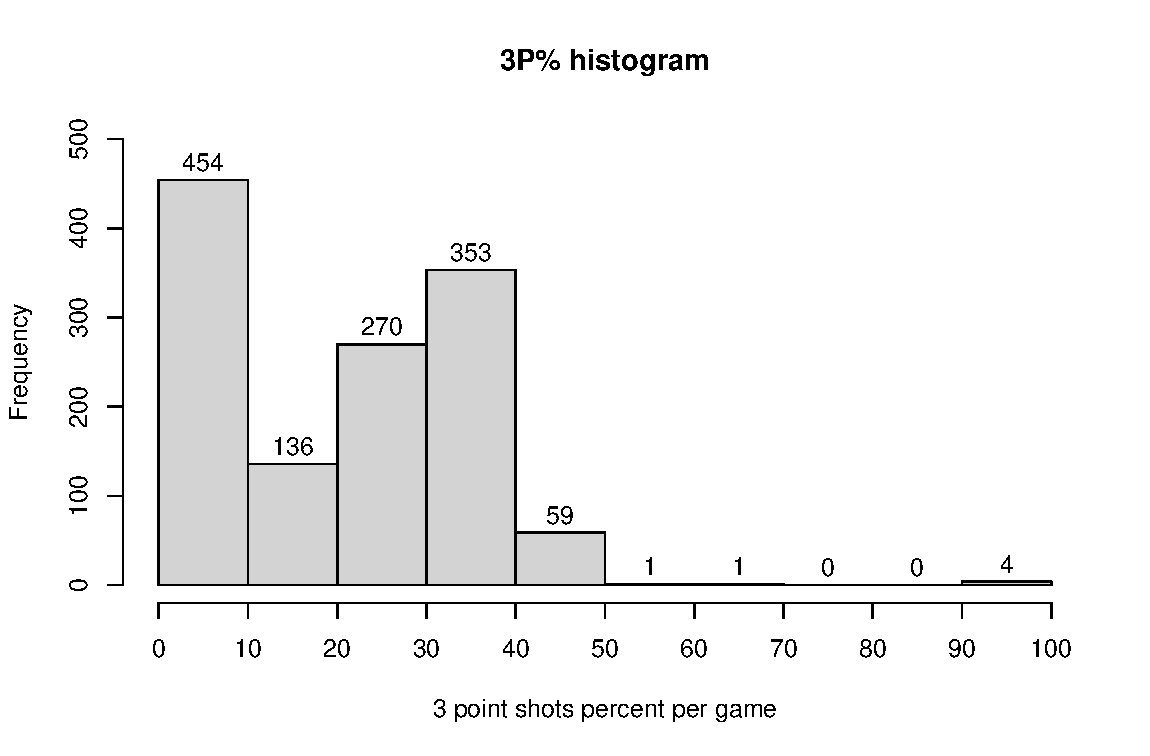
\includegraphics[width=0.5\linewidth]{ImageFiles/Histograms/histogram_x3p.pdf}
		\caption{}
		\label{fig:HistX3P}
	\end{subfigure}
	\begin{subfigure}{.3\textwidth}
		\centering
		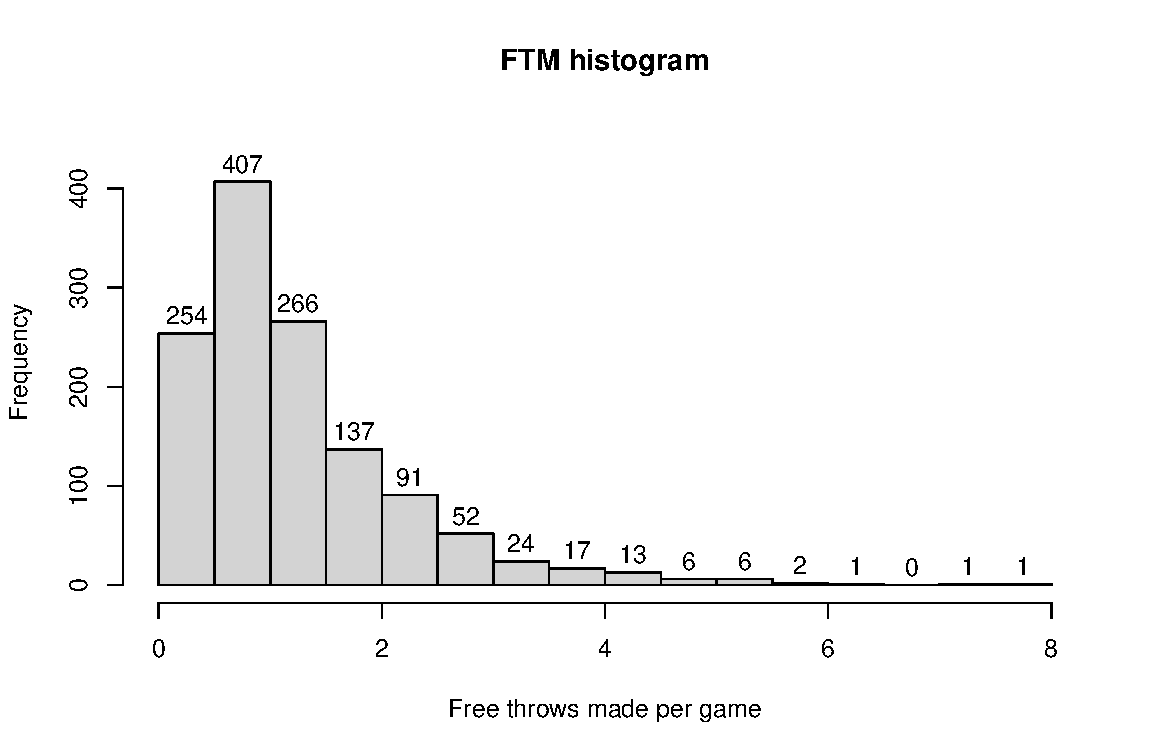
\includegraphics[width=0.5\linewidth]{ImageFiles/Histograms/histogram_ftm.pdf}
		\caption{}
		\label{fig:HistFTM}
	\end{subfigure}%
	\begin{subfigure}{.3\textwidth}
		\centering
		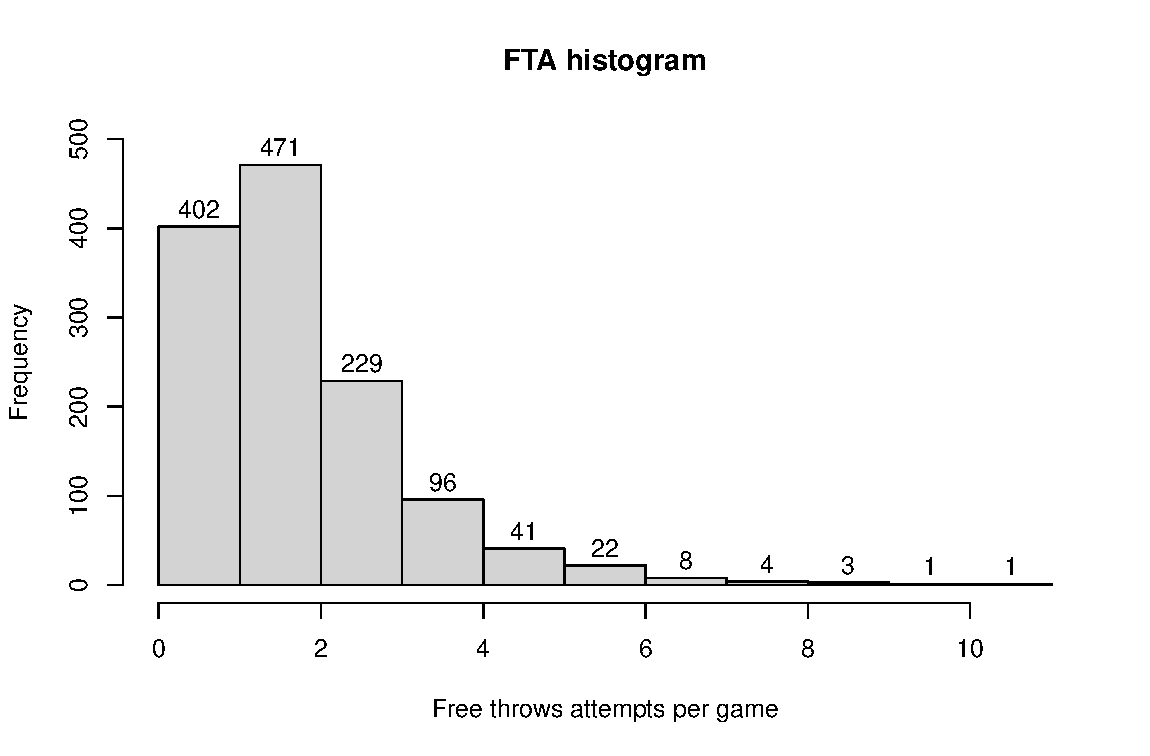
\includegraphics[width=0.5\linewidth]{ImageFiles/Histograms/histogram_fta.pdf}
		\caption{}
		\label{fig:HistFTA}
	\end{subfigure}%
	\begin{subfigure}{.3\textwidth}
		\centering
		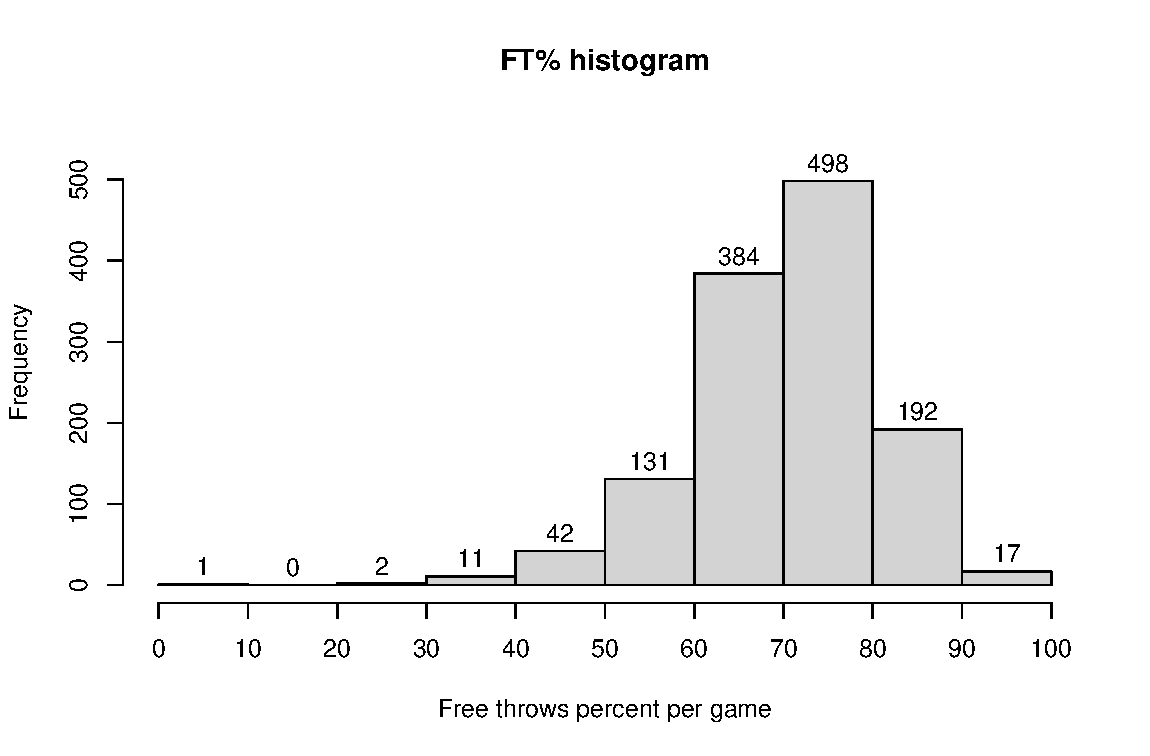
\includegraphics[width=0.5\linewidth]{ImageFiles/Histograms/histogram_ft.pdf}
		\caption{}
		\label{fig:HistFT}
	\end{subfigure}
	\begin{subfigure}{.3\textwidth}
		\centering
		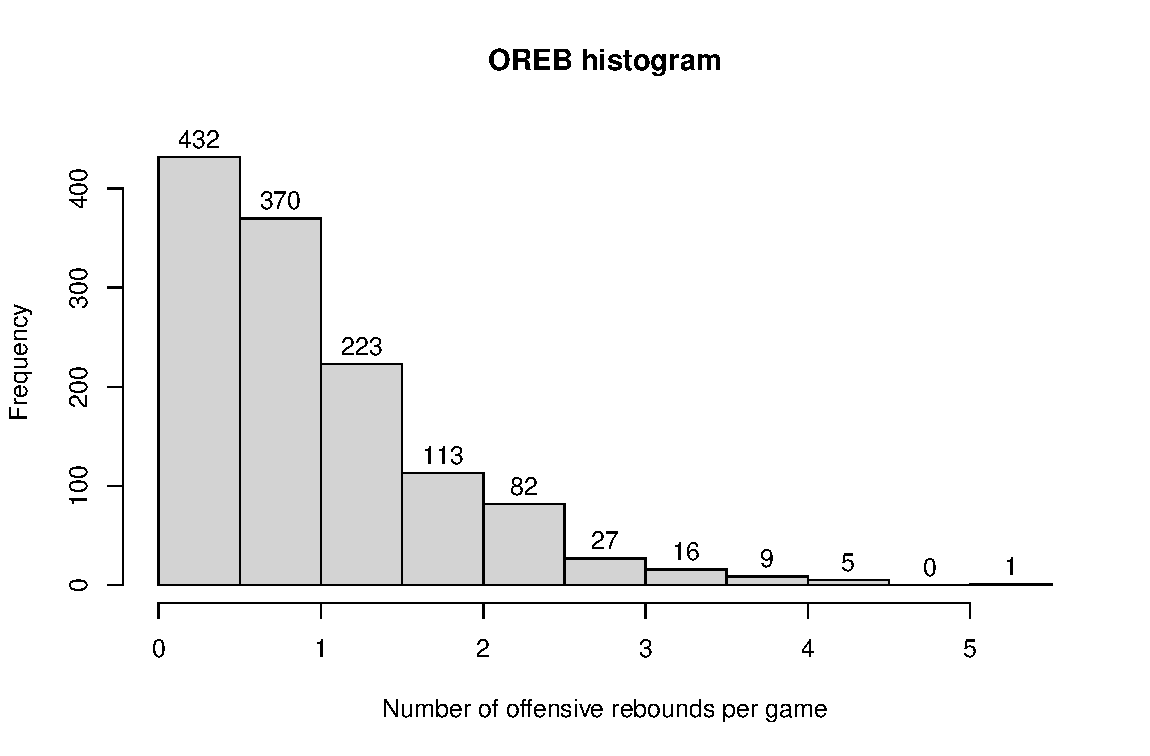
\includegraphics[width=0.5\linewidth]{ImageFiles/Histograms/histogram_oreb.pdf}
		\caption{}
		\label{fig:HistOREB}
	\end{subfigure}%
	\begin{subfigure}{.3\textwidth}
		\centering
		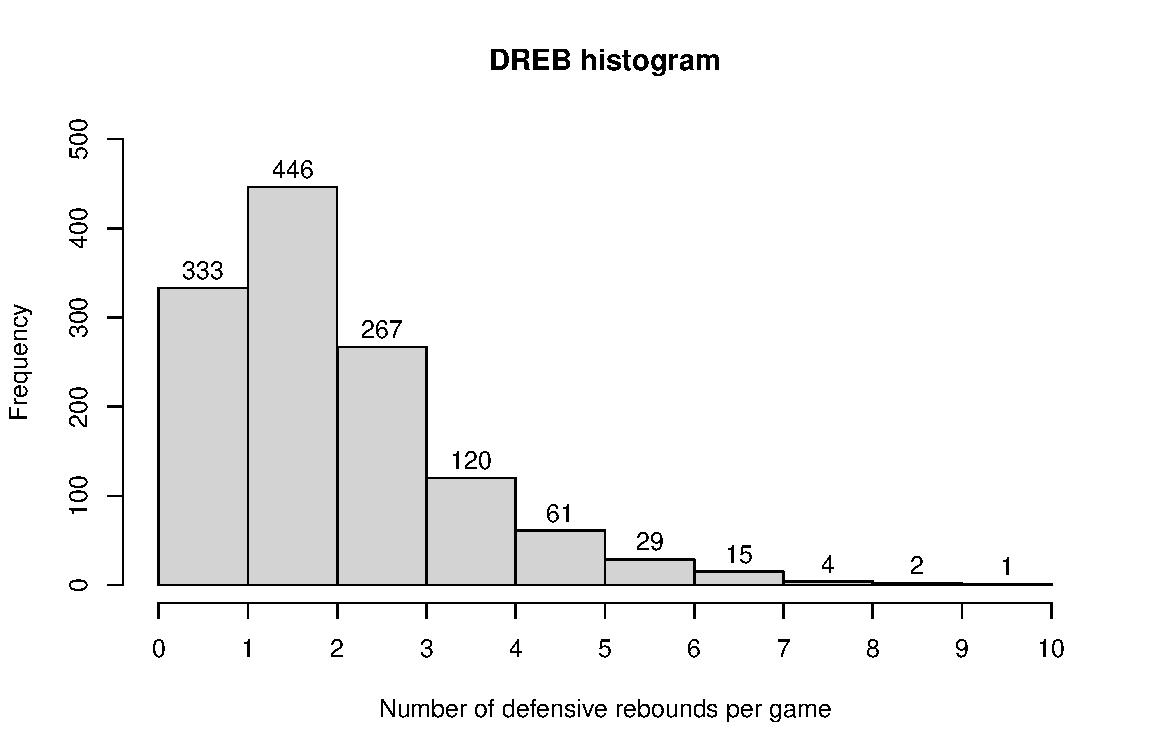
\includegraphics[width=0.5\linewidth]{ImageFiles/Histograms/histogram_dreb.pdf}
		\caption{}
		\label{fig:HistDREB}
	\end{subfigure}%
	\begin{subfigure}{.3\textwidth}
		\centering
		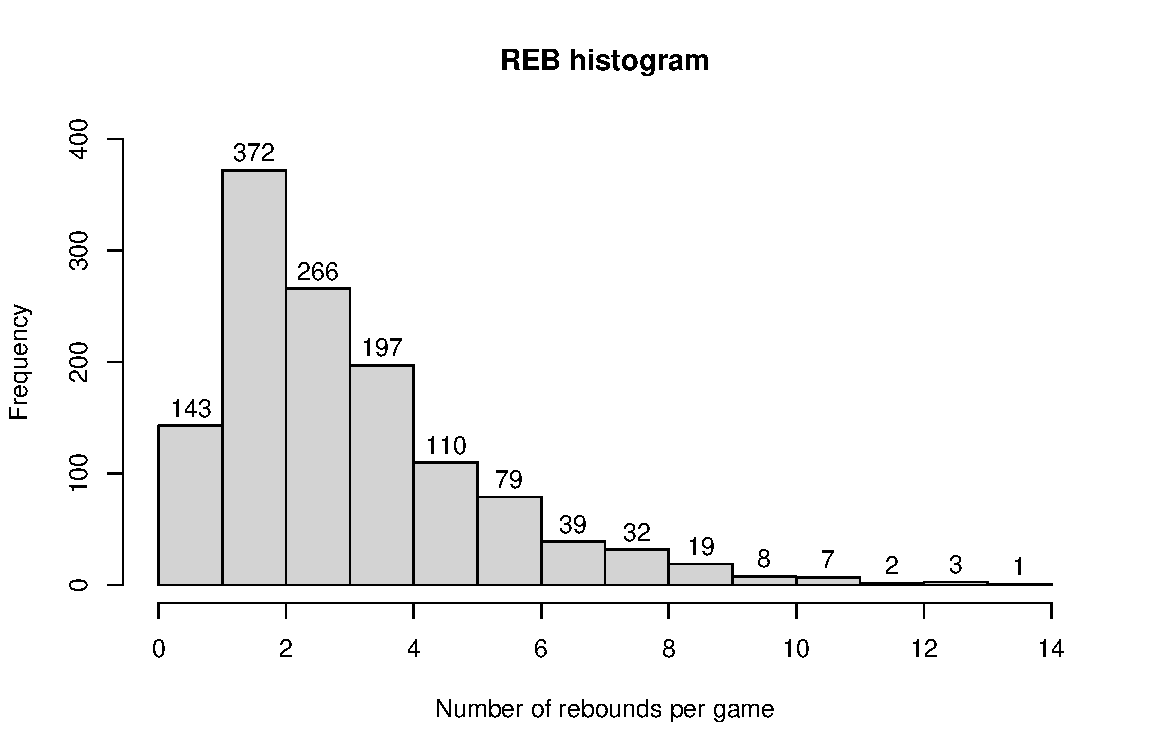
\includegraphics[width=0.5\linewidth]{ImageFiles/Histograms/histogram_reb.pdf}
		\caption{}
		\label{fig:HistREB}
	\end{subfigure}
	\begin{subfigure}{.3\textwidth}
		\centering
		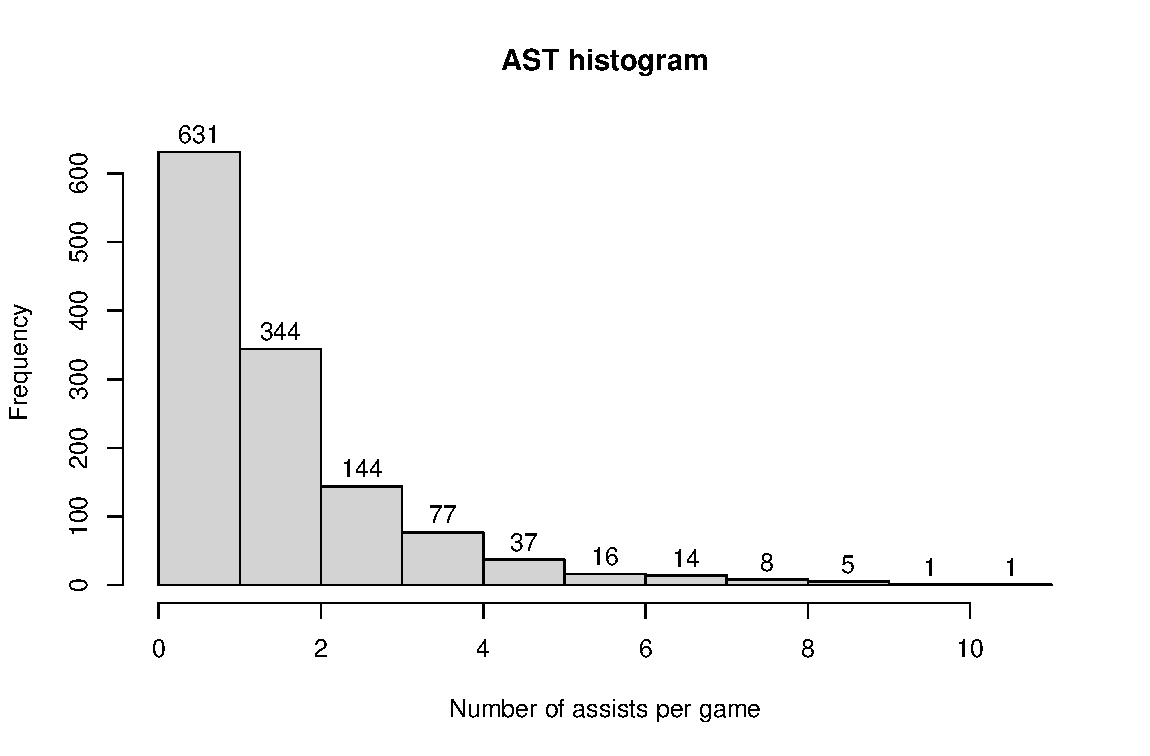
\includegraphics[width=0.5\linewidth]{ImageFiles/Histograms/histogram_ast.pdf}
		\caption{}
		\label{fig:HistAST}
	\end{subfigure}%
	\begin{subfigure}{.3\textwidth}
		\centering
		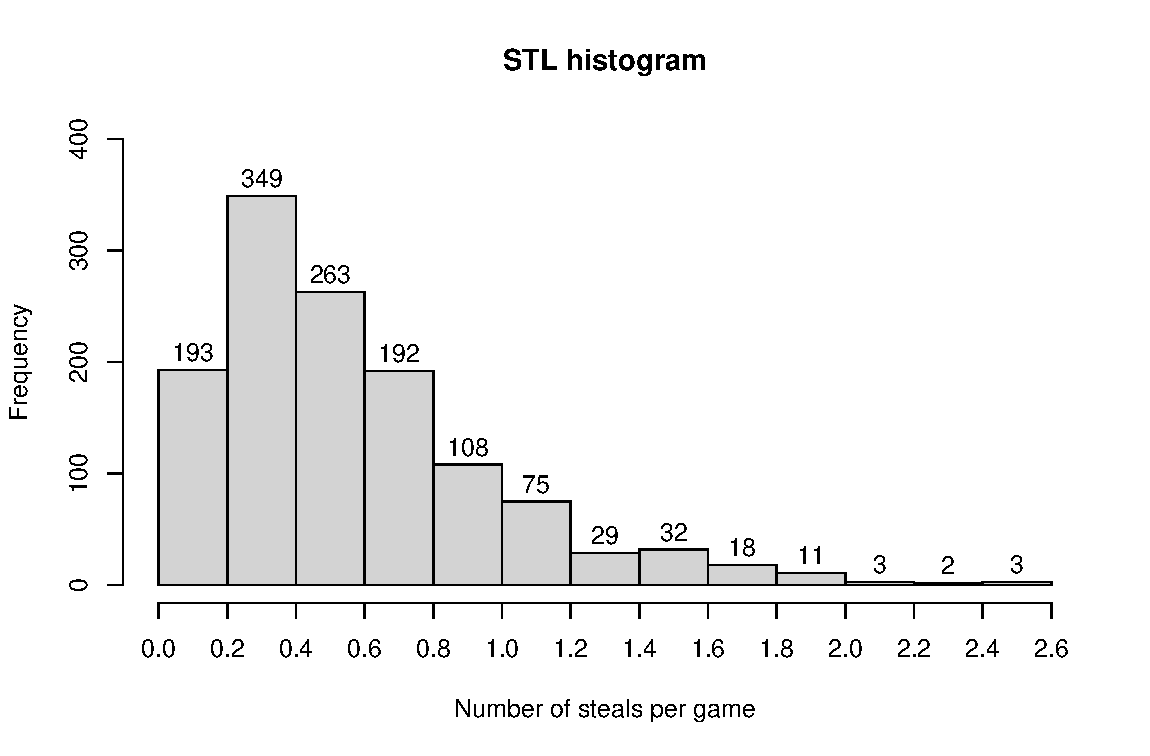
\includegraphics[width=0.5\linewidth]{ImageFiles/Histograms/histogram_stl.pdf}
		\caption{}
		\label{fig:HistSTL}
	\end{subfigure}%
	\begin{subfigure}{.3\textwidth}
		\centering
		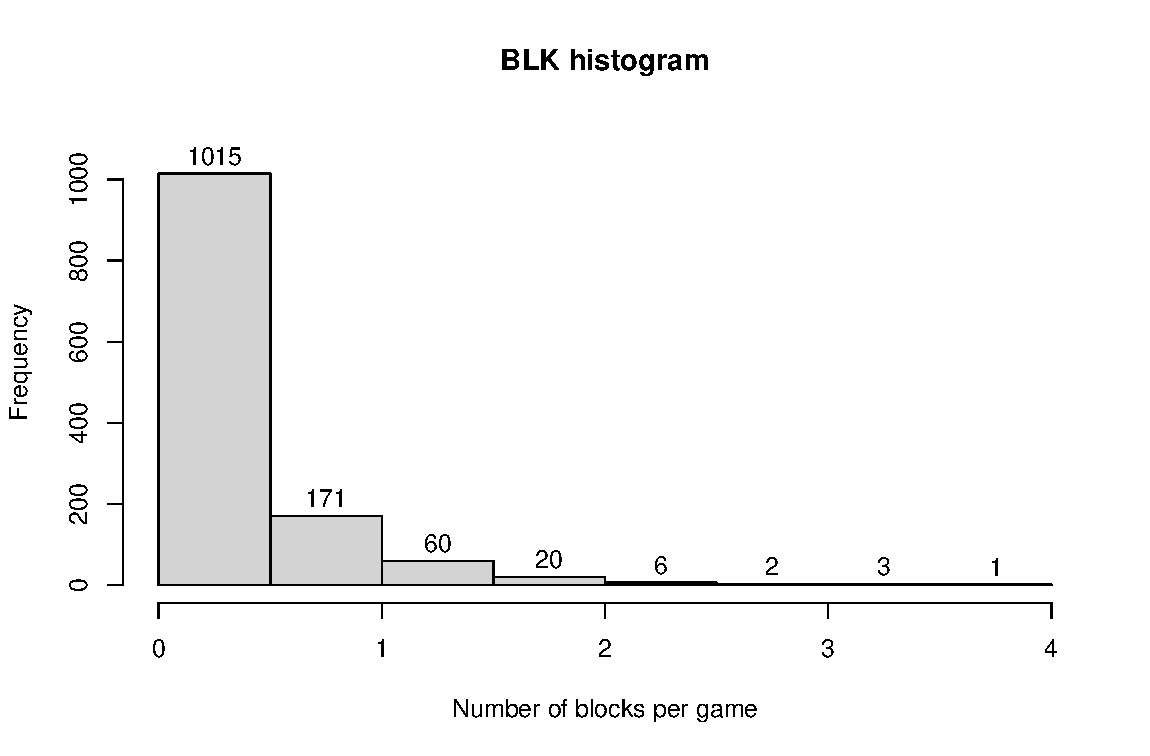
\includegraphics[width=0.5\linewidth]{ImageFiles/Histograms/histogram_blk.pdf}
		\caption{}
		\label{fig:HistBLK}
	\end{subfigure}
	\begin{subfigure}{.3\textwidth}
		\centering
		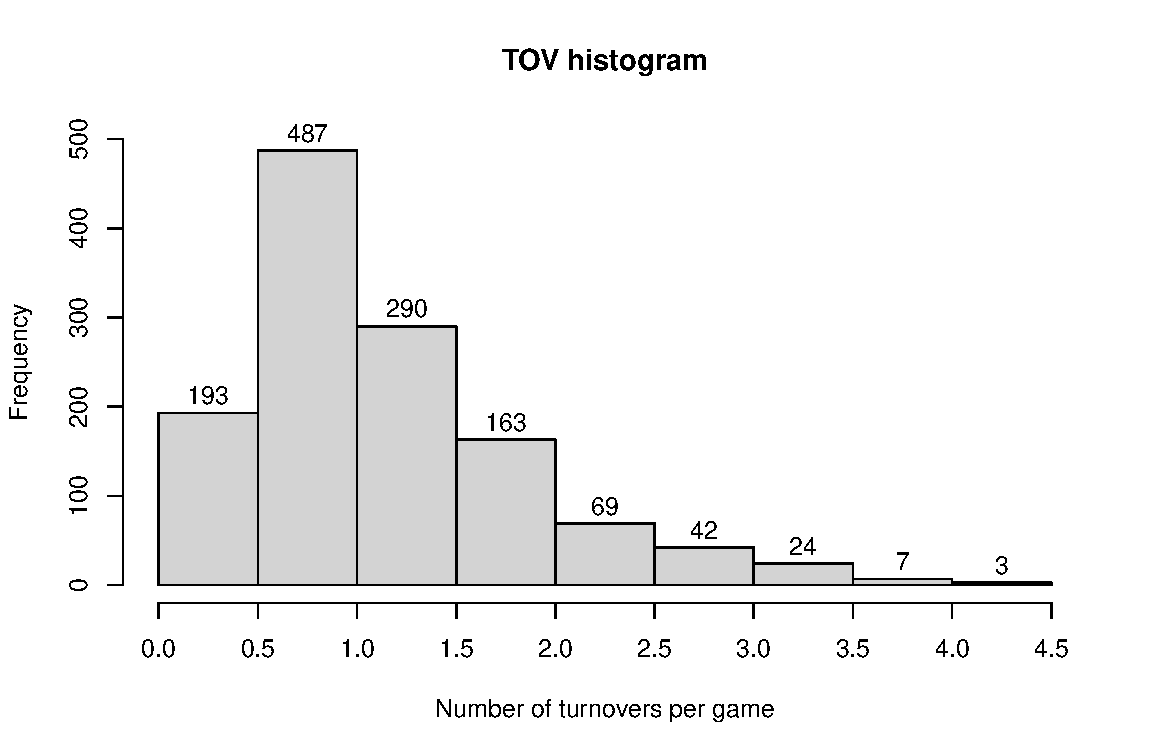
\includegraphics[width=0.5\linewidth]{ImageFiles/Histograms/histogram_tov.pdf}
		\caption{}
		\label{fig:HistTOV}
	\end{subfigure}
	\caption{Variables histograms.}
	\label{fig:Histograms}
\end{figure}

We can also look at the output variable to check whether the dataset was balanced or not. In \Fig~\ref{fig:target_bar_plot} we can clearly see that the samples are not equally distributed. 

\begin{figure}[H]
	\centering
	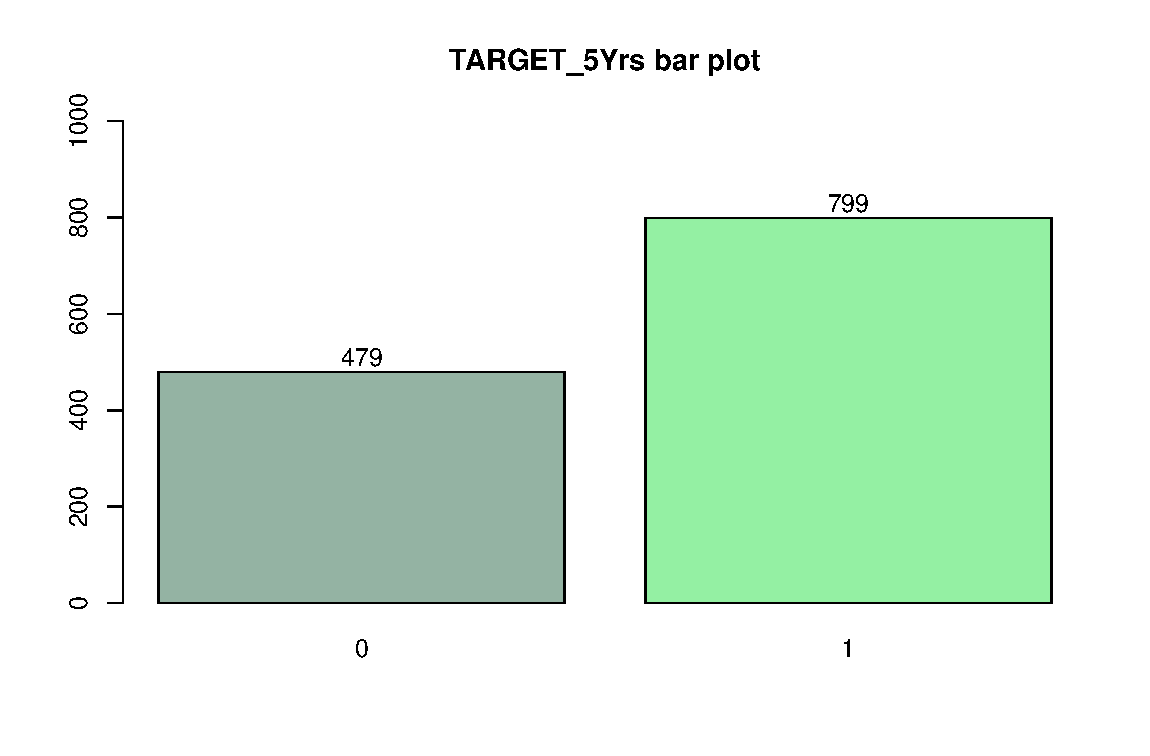
\includegraphics[width=0.5\linewidth]{ImageFiles/Histograms/bp_target5yrs.pdf}
	\caption{Target variable bar plot.}
	\label{fig:target_bar_plot}
\end{figure}

\textbf{Scientific questions}
\begin{itemize}
	\item What are the key contributing factors that significantly influence a player's ability to score points at a high level?
	\item Is it true that a player's career length increase based only on scoring more points?
\end{itemize}

\noindent
The objective of this analysis is to develop two distinct models that can effectively explain the variables ``PTS'' and ``TARGET\_5Yrs''. 
 
Due to its continuous nature, ``PTS'' necessitates the use of regression methods. We intend to employ a linear regression model, incorporating various model selection algorithms such as subset selection and regularization.

Instead, as ``TARGET\_5Yrs'' represents a categorical variable, it calls for the application of classification techniques. Our approach involves exploring various classification models, including logistic regression, tree-based methods, k-nearest neighbors, and support vector machines.

All the techniques employed are obtained from \cite{James2013}.